Netty è un framework NIO (Non-blocking Input Output) di tipo client-server (i.e. permette una comunicazione asincrona tra client e server di tipo event-driven) che facilita lo sviluppo di applicazioni di rete che utilizzano socket TCP e UDP.

Il framework è disponibile sul Maven Central Repository e può essere scaricato includendo la seguente dependency nel pom.xml del progetto:
\begin{lstlisting} [caption={My Caption},captionpos=b]
<dependencies>
	<dependency>
		<groupId>io.netty</groupId>
		<artifactId>netty-all</artifactId>
		<version>4.1.32.Final</version>
	</dependency>
</dependencies>
\end{lstlisting}

Lato Server creiamo un oggetto singleton di tipo \textit{Communication} il quale inizializza a sua volte un oggetto di tipo \textit{ServerBootstrap} (io.netty.bootstrap.ServerBootstrap).

Quest'ultimo effettua il bootstrap del \textit{ServerChannel}, dove il \textit{ServerChannel} rappresenta il link "primario" (sul port 5000) che accetta ogni connessione di un client e crea un canale "figlio" sul quale avverà tale comunicazione.

\begin{lstlisting} [caption={My Caption},captionpos=b]
private Communication() throws Exception {
	ServerBootstrap b = new ServerBootstrap();

	b.group(bossGroup, workerGroup).channel(NioServerSocketChannel.class).handler(new LoggingHandler(LogLevel.INFO)).childHandler(new ServerInitializer(sslCtx));

	b.bind(PORT).sync().channel().closeFuture().sync();
}
\end{lstlisting}
\newpage
Al server andiamo ad aggiungere un handler \textit{ServerInitializer} che aggiunge alla pipeline, oltre agli encoder e decoder di default, il \textit{ServerHandler}.

\begin{lstlisting} [caption={My Caption},captionpos=b]
class ServerInitializer extends ChannelInitializer<SocketChannel> {

	private static final StringDecoder DECODER = new StringDecoder();
	private static final StringEncoder ENCODER = new StringEncoder();
	private static final ServerHandler SERVER_HANDLER = new ServerHandler();
	
	@Override
	public void initChannel(SocketChannel ch) throws Exception {
		ChannelPipeline pipeline = ch.pipeline();
		pipeline.addLast(DECODER);
		pipeline.addLast(ENCODER);
		// and then business logic.
		pipeline.addLast(SERVER_HANDLER);
	}
}
\end{lstlisting}

La classe \textit{ServerHandler} è un sottotipo di \textit{SimpleChannelInboundHandler} \\(io.netty.channel.SimpleChannelInboundHandler) il quale fornisce la stringa inviata dal client tramite il metodo seguente.

\begin{lstlisting} [caption={My Caption},captionpos=b]
class ServerHandler extends SimpleChannelInboundHandler<String> {
	
	@Override
	public void channelRead0(ChannelHandlerContext ctx, String request) throws Exception {
		int j = request.indexOf(";");
		String username = request.substring(0, j);
		Communication.chcMap.put(username, ctx);
		
		System.out.println("Process request: " + request);
		computeRequest.process(request.substring(j + 1), username);
	}
}
\end{lstlisting}

Si può notare che il metodo precedente memorizza la coppia (username, \textit{channelHandlerContext}) all'interno dell'oggetto chcMap di \textit{Communication}, il quale è di tipo HashMap<String, ChannelHandlerContext>.
Tale informazione è fondamentale al fine di rispondere al client tramite canale "figlio" ad esso dedicato e chiuderlo al termine della comunicazione: il metodo invoca poi l'elaborazione del messaggio ricevuto tramite l'interfaccia \textit{ProcessRequest} (la semantica della stringa request verrà discussa nel paragrafo successivo).

\newpage
Infine, ma non per importanza, discutiamo l'implementazione dell'interfaccia \textit{SendAnswer} da parte della classe \textit{Communication}:
\begin{lstlisting}[caption={My Caption},captionpos=b]
public final class Communication implements SendAnswer{

	public void send(final String username, final String msg) {	
		ChannelFuture oo = chcMap.get(username).writeAndFlush(msg + "\r\n");
		oo.addListener(new ChannelFutureListener() {
		
			public void operationComplete(ChannelFuture future)	throws Exception {
				int count = 0;
				boolean isError = false;
				
				while(!future.isSuccess()) {
					chcMap.get(username).writeAndFlush(msg + "\r\n");
					System.out.println("Retry send response!");
					if(count == 3) {
						isError = true;
						break;
					} else {
						count ++;
					}
				}
				
				future.addListener(ChannelFutureListener.CLOSE);
				chcMap.remove(username);
			}
		});
	}
}
\end{lstlisting}

Il metodo Send, definito all'interno della classe \textit{Communication}, si occupa di inviare la risposta relativa alla richiesta ricevuta e, nel caso di fallimento, ripeterà l'invio fino a un limite di 3 tentativi.
\begin{figure}[h]
	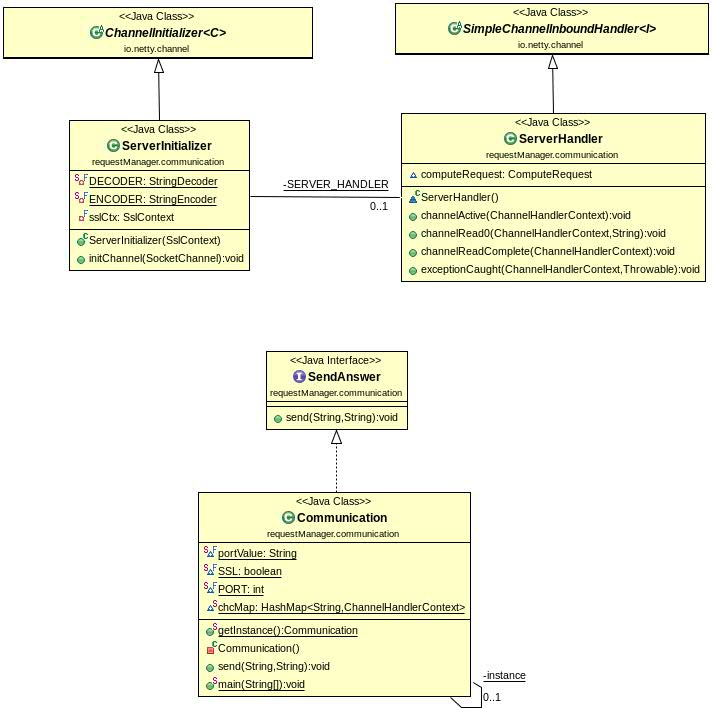
\includegraphics[width=\textwidth]{Immagini/CommunicationPackageServer}
	\caption{Struttura del package \textit{requestManager.Communication}}
	\label{fig:requestManager}
\end{figure}
\newpage
Lato Client creiamo un oggetto singleton \textit{Communication} che implementa il seguente metodo dell'interfaccia \textit{SendRequest}, aprendo la connessione con il Server sulla socket (35.180.103.132,5000) e inviando il messaggio al server.

\begin{lstlisting}[caption={My Caption},captionpos=b]
public class Communication implements SendRequest {
	private static final String IP = "35.180.103.132";
	public static final String HOST = System.getProperty("host", IP);
	public static final int PORT = 5000;
	@Override
	public boolean send(String data) {
		Bootstrap b = new Bootstrap();
		b.group(group).channel(NioSocketChannel.class).handler(new ClientInitializer(sslCtx));
		ChannelFuture ch = null;
		
		ch = b.connect(HOST, PORT);
		
		ChannelFuture lastWriteFuture = null;
		lastWriteFuture = ch.channel().writeAndFlush(data + "\r\n");
		
		//Wait until all messages are flushed before closing the channel
		if (lastWriteFuture != null) {
			lastWriteFuture.sync();
		}		
	}
}
\end{lstlisting}

Tralasciando la discussione dell'implementazione della classe \textit{ClientInitializer} in quanto simile a quella della classe duale lato server.

Andiamo invece ad approfondire l'implementazione della classe \textit{ClientHandler}:.

\begin{lstlisting}[caption={My Caption},captionpos=b]
class ClientHandler extends SimpleChannelInboundHandler<String> {
	@Override
	protected void channelRead0(ChannelHandlerContext ctx, String msg) {
		Processing.getInstance().processAnswer(msg);
		Communication.getInstance().group.shutdownGracefully();
	}
}
\end{lstlisting}

Di particolare interesse è il metodo \textit{channelRead0} ereditato da \textit{SimpleChannelInboundHandler}, il quale viene invocato dal framework ogni qual volta il client riceve un messaggio.

Il messaggio viene poi elaborato dal oggetto singleton \textit{Processing} e il canale di comunicazione viene chiuso.

\begin{figure}[h]
	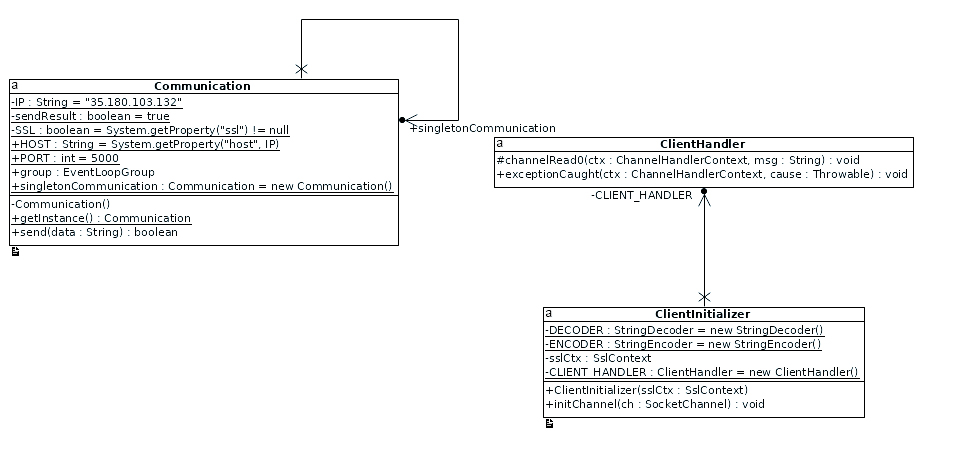
\includegraphics[width=\textwidth]{Immagini/CommunicationPackageClient}
	\caption{Struttura del package \textit{requestManager.Communication}}
	\label{fig:requestManagerCommunication}
\end{figure}







